


\begin{figure}[t!]
    \centering
    \begin{subfigure}[t]{0.325\textwidth}
        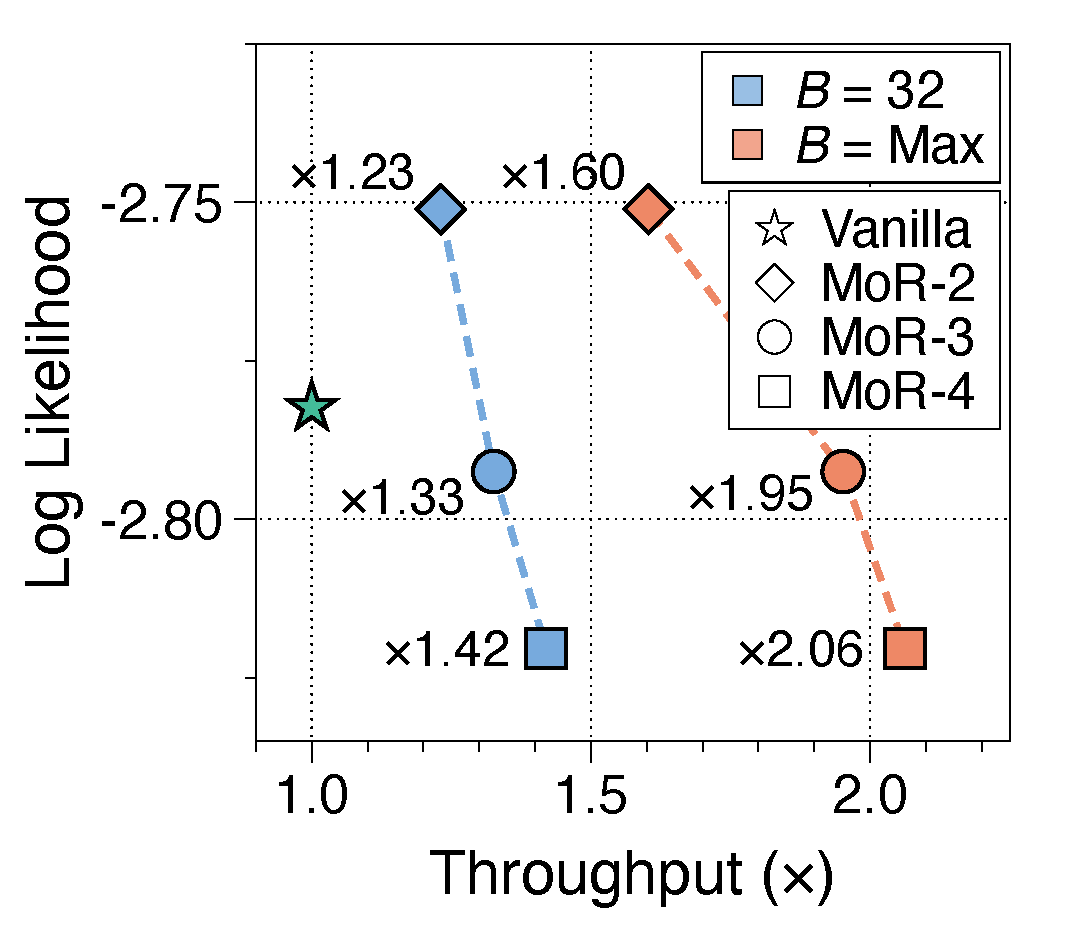
\includegraphics[width=\textwidth]{figs/throughput/throughput_256.pdf}
        \captionsetup{justification=centering}
        \subcaption{Pareto frontier of throughput}
        \label{fig:pareto_frontier_sharing-a}
    \end{subfigure}
    \centering
    \begin{subfigure}[t]{0.325\textwidth}
        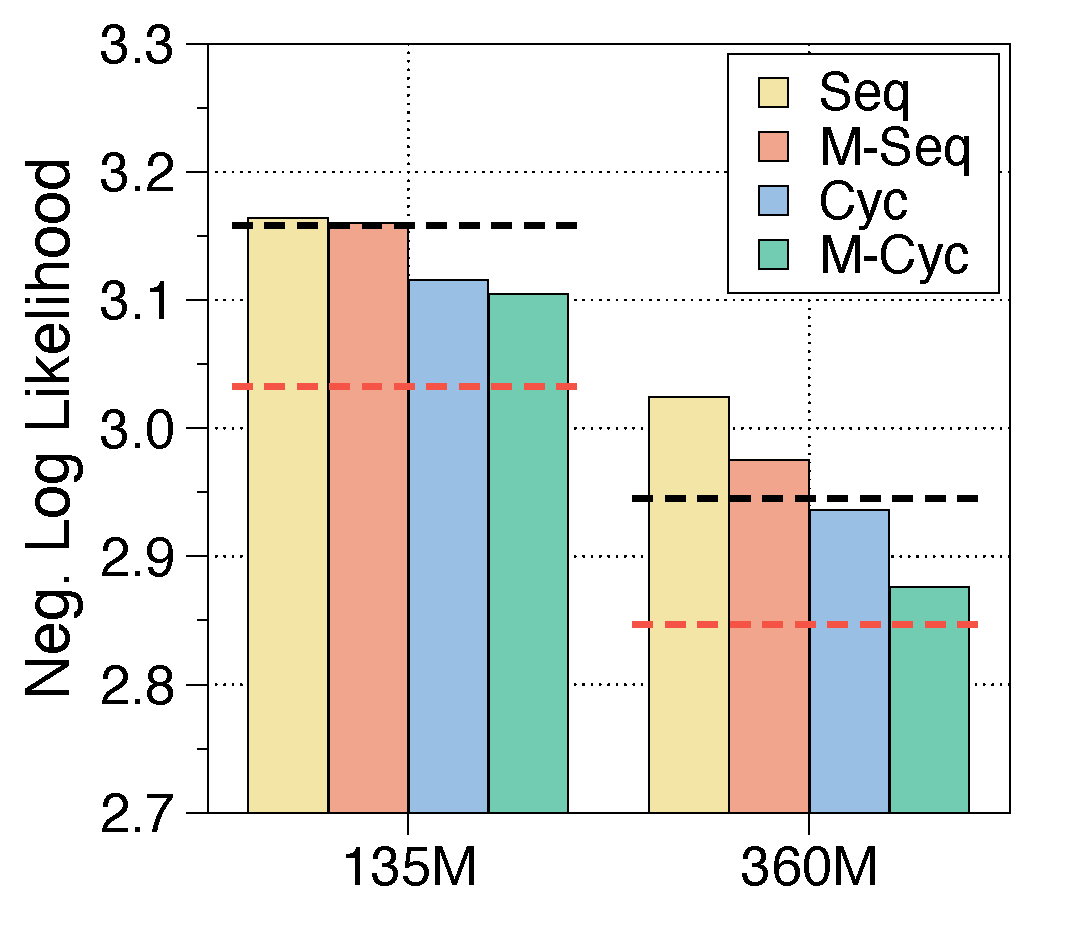
\includegraphics[width=\textwidth]{figs/revisit_sharing/revisit_sharing_rec3.pdf}
        \captionsetup{justification=centering}
        \subcaption{Sharing strategy}
        \label{fig:pareto_frontier_sharing-b}
    \end{subfigure}
    \begin{subfigure}[t]{0.325\textwidth}
        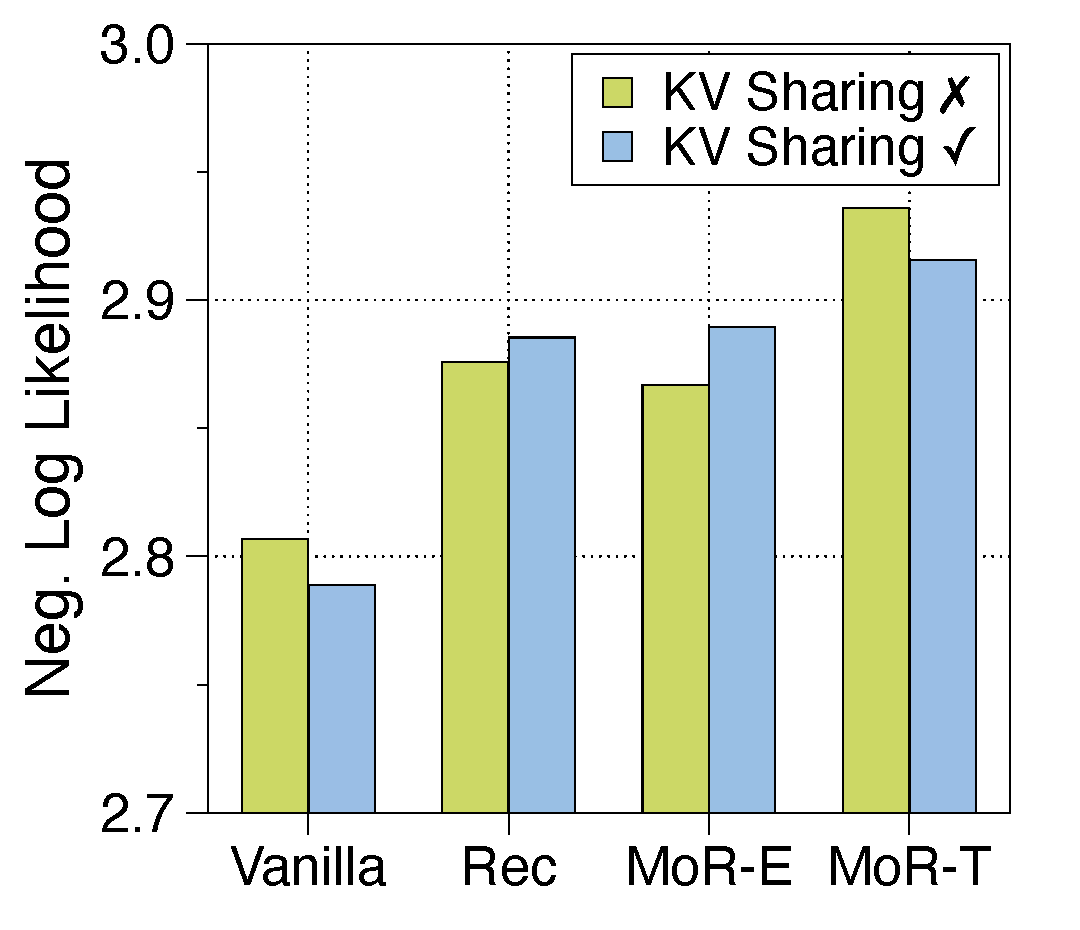
\includegraphics[width=\textwidth]{figs/kv_sharing/kv_sharing_loss.pdf}
        \captionsetup{justification=centering}
        \subcaption{KV cache sharing}
        \label{fig:pareto_frontier_sharing-c}
    \end{subfigure}
    \centering
    \caption{
    (a) Pareto frontier of inference throughput and log-likehood for MoR and Vanilla Transformer under fixed and maximum batching scenarios. Setting details are in \autoref{app:throughput}.
    (b) Negative log-likelihood (NLL) of Recursive Transformers with $N_r=3$ across four different parameter-sharing strategies. We pretrained the models on 10 billion tokens. The dashed red and black lines denote the full-size Vanilla Transformer and parameter-matched vanilla models (approximately one-third scales), respectively.
    (c) NLL performance comparison across four different architectures with KV sharing. 
    For MoR, green (disabled) and blue (enabled) refer to recursion-wise KV caching and recursive KV sharing strategies. MoR-E and MoR-T denotes expert-choice and token-choice MoR, respectively. All models are based on 360M scale and trained on 10 billion tokens.\looseness=-1
    }    
    \label{fig:pareto_frontier_sharing}
\end{figure}